\chapter{Experiments}
\label{chap:experiments}
This chapter presents the experiments designed to evaluate the system described in chapter \autoref{chap:methods}.
The chapter is structured as follows: \autoref{sec:exp-setup} specifies the setup used for the class incremental learning task; \autoref{sec:exp-cil} discusses the experiments related to the CIL model and \autoref{sec:exp-det} those related to the logo detector; \autoref{sec:exp-kd} describes the experiments relative to the KD; finally, \autoref{sec:exp-end2end} presents the results of experiments combining the logo detector with the CIL classifier.

\section{Setup}
\label{sec:exp-setup}
The developed system is tested considering two different CIL setups: in the first setup, the system is tested on a subset of 100 classes out of the total 2993 in the dataset; in the second setup, the model's scaling capabilities are tested considering the entire dataset. Specifically, the CIL configuration is the following:
\begin{enumerate}
    \item \textbf{100 Classes}: 100 classes are extracted from the initial dataset. For the experiments, a distinction is made between the case in which these classes are extracted randomly or are taken the 100 classes with the highest number of images.
    
    Out of these 100 classes, 30 are used for the initial task, then the remaining 70 classes are added 10 at a time through 7 incremental learning iterations.

    \item \textbf{2993 Classes (entire dataset)}: for experiments which consider the entire dataset, the first 1000 classes are used for the initial task, then follows 8 iterations of incremental learning, each adding 250 new classes.
\end{enumerate}

The train, validation and test set are built from the individual classes. For each of these, the instances are divided as follows:
\begin{itemize}
    \item \textbf{Train set}: 70 \%
    \item \textbf{Validation set}: 10 \%
    \item \textbf{Test set}: 20 \%
\end{itemize}


\section{Classifier: CIL model}
\label{sec:exp-cil}
Top-k accuracy is used to evaluate the performance of the CIL model, focusing on cases with $k=1$ and $k=5$.
Using this performance metric, a classification is considered correct if the label is present among the first $k$ predictions to which the model assigns the highest probability. Thus, the accuracy is calculated as the percentage of the correct predictions.

\subsection{100 Classes}
\subsubsection{100 Classes randomly sampled}
For the first experiments, the 100 classes are randomly sampled from the 2993 classes in the dataset, then the classifier is evaluated on the test set according to the CIL setup described in \autoref{sec:exp-setup}. 

As detailed in \autoref{sec:der-algorithm}, the DER algorithm saves some examples of the 'old' classes and reuses these examples during incremental learning iterations. In the following experiments, the memory dedicated to each old class is of 100 samples.

The first group of experiments aims to compare two types of architecture: ResNet-34 and ResNet-50. In addition, the cases where CNNs are pre-trained on ImageNet or not are also considered. For these experiments, the optimizer is SGD and neither regularization of the model via the dropout layer nor data augmentation is used.

The results of the experiments in picture \autoref{fig:exp1} and table \autoref{table:exp1}, reporting the top-1 and top-5 accuracy of the models at varying CIL tasks on the test set, show that pre-trained CNNs perform better, but there is not much difference between ResNet-34 and ResNet-50. For this reason, the architecture chosen for the experiments to follow is ResNet-34, so as to have a slightly smaller network than ResNet-50, and the network is pre-trained on ImageNet.

Other useful insights can be derived from the training history of a task (e.g. Task 7) which reports the top-1 accuracy on the training and validation set. In fact, as we can see from \autoref{fig:exp1-train_val} the accuracy on the training set is much higher than the validation set, which is a clear sign of overfitting of the model.

\begin{figure}[H]
	\centering
	\subfloat[\centering Top-1 accuracy]{{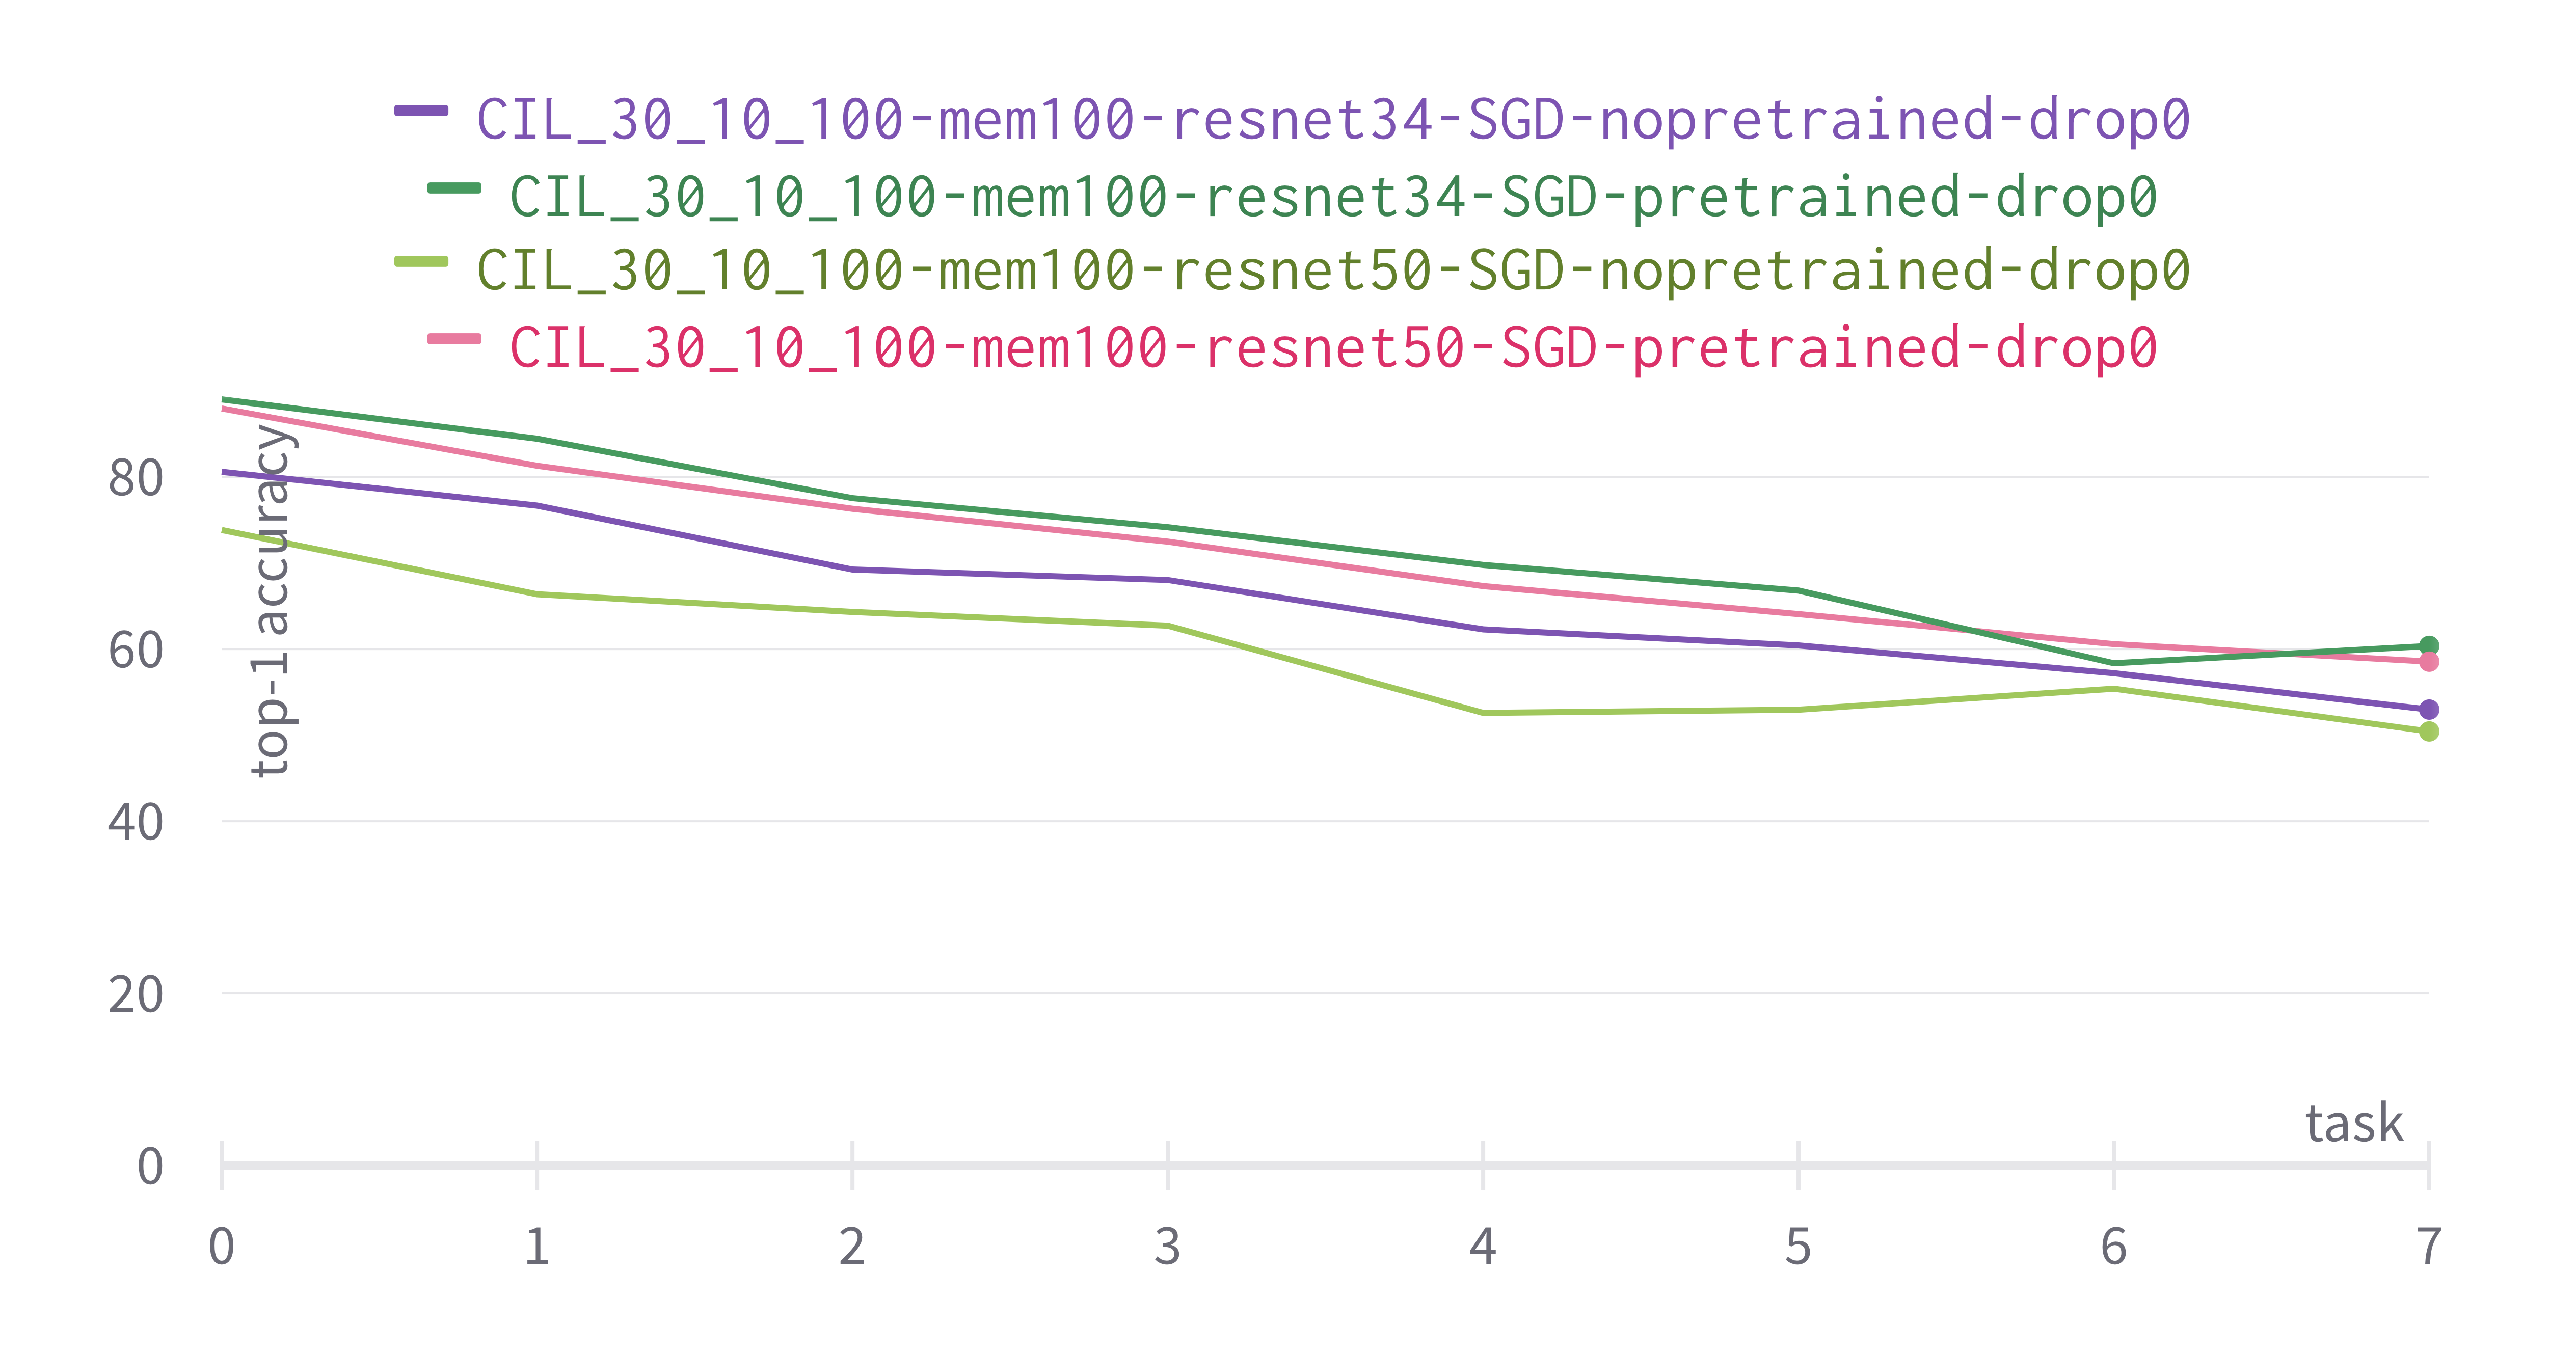
\includegraphics[width=0.50\textwidth]{images/exp/exp1-top1.png} }}%
	\subfloat[\centering Top-5 accuracy]{{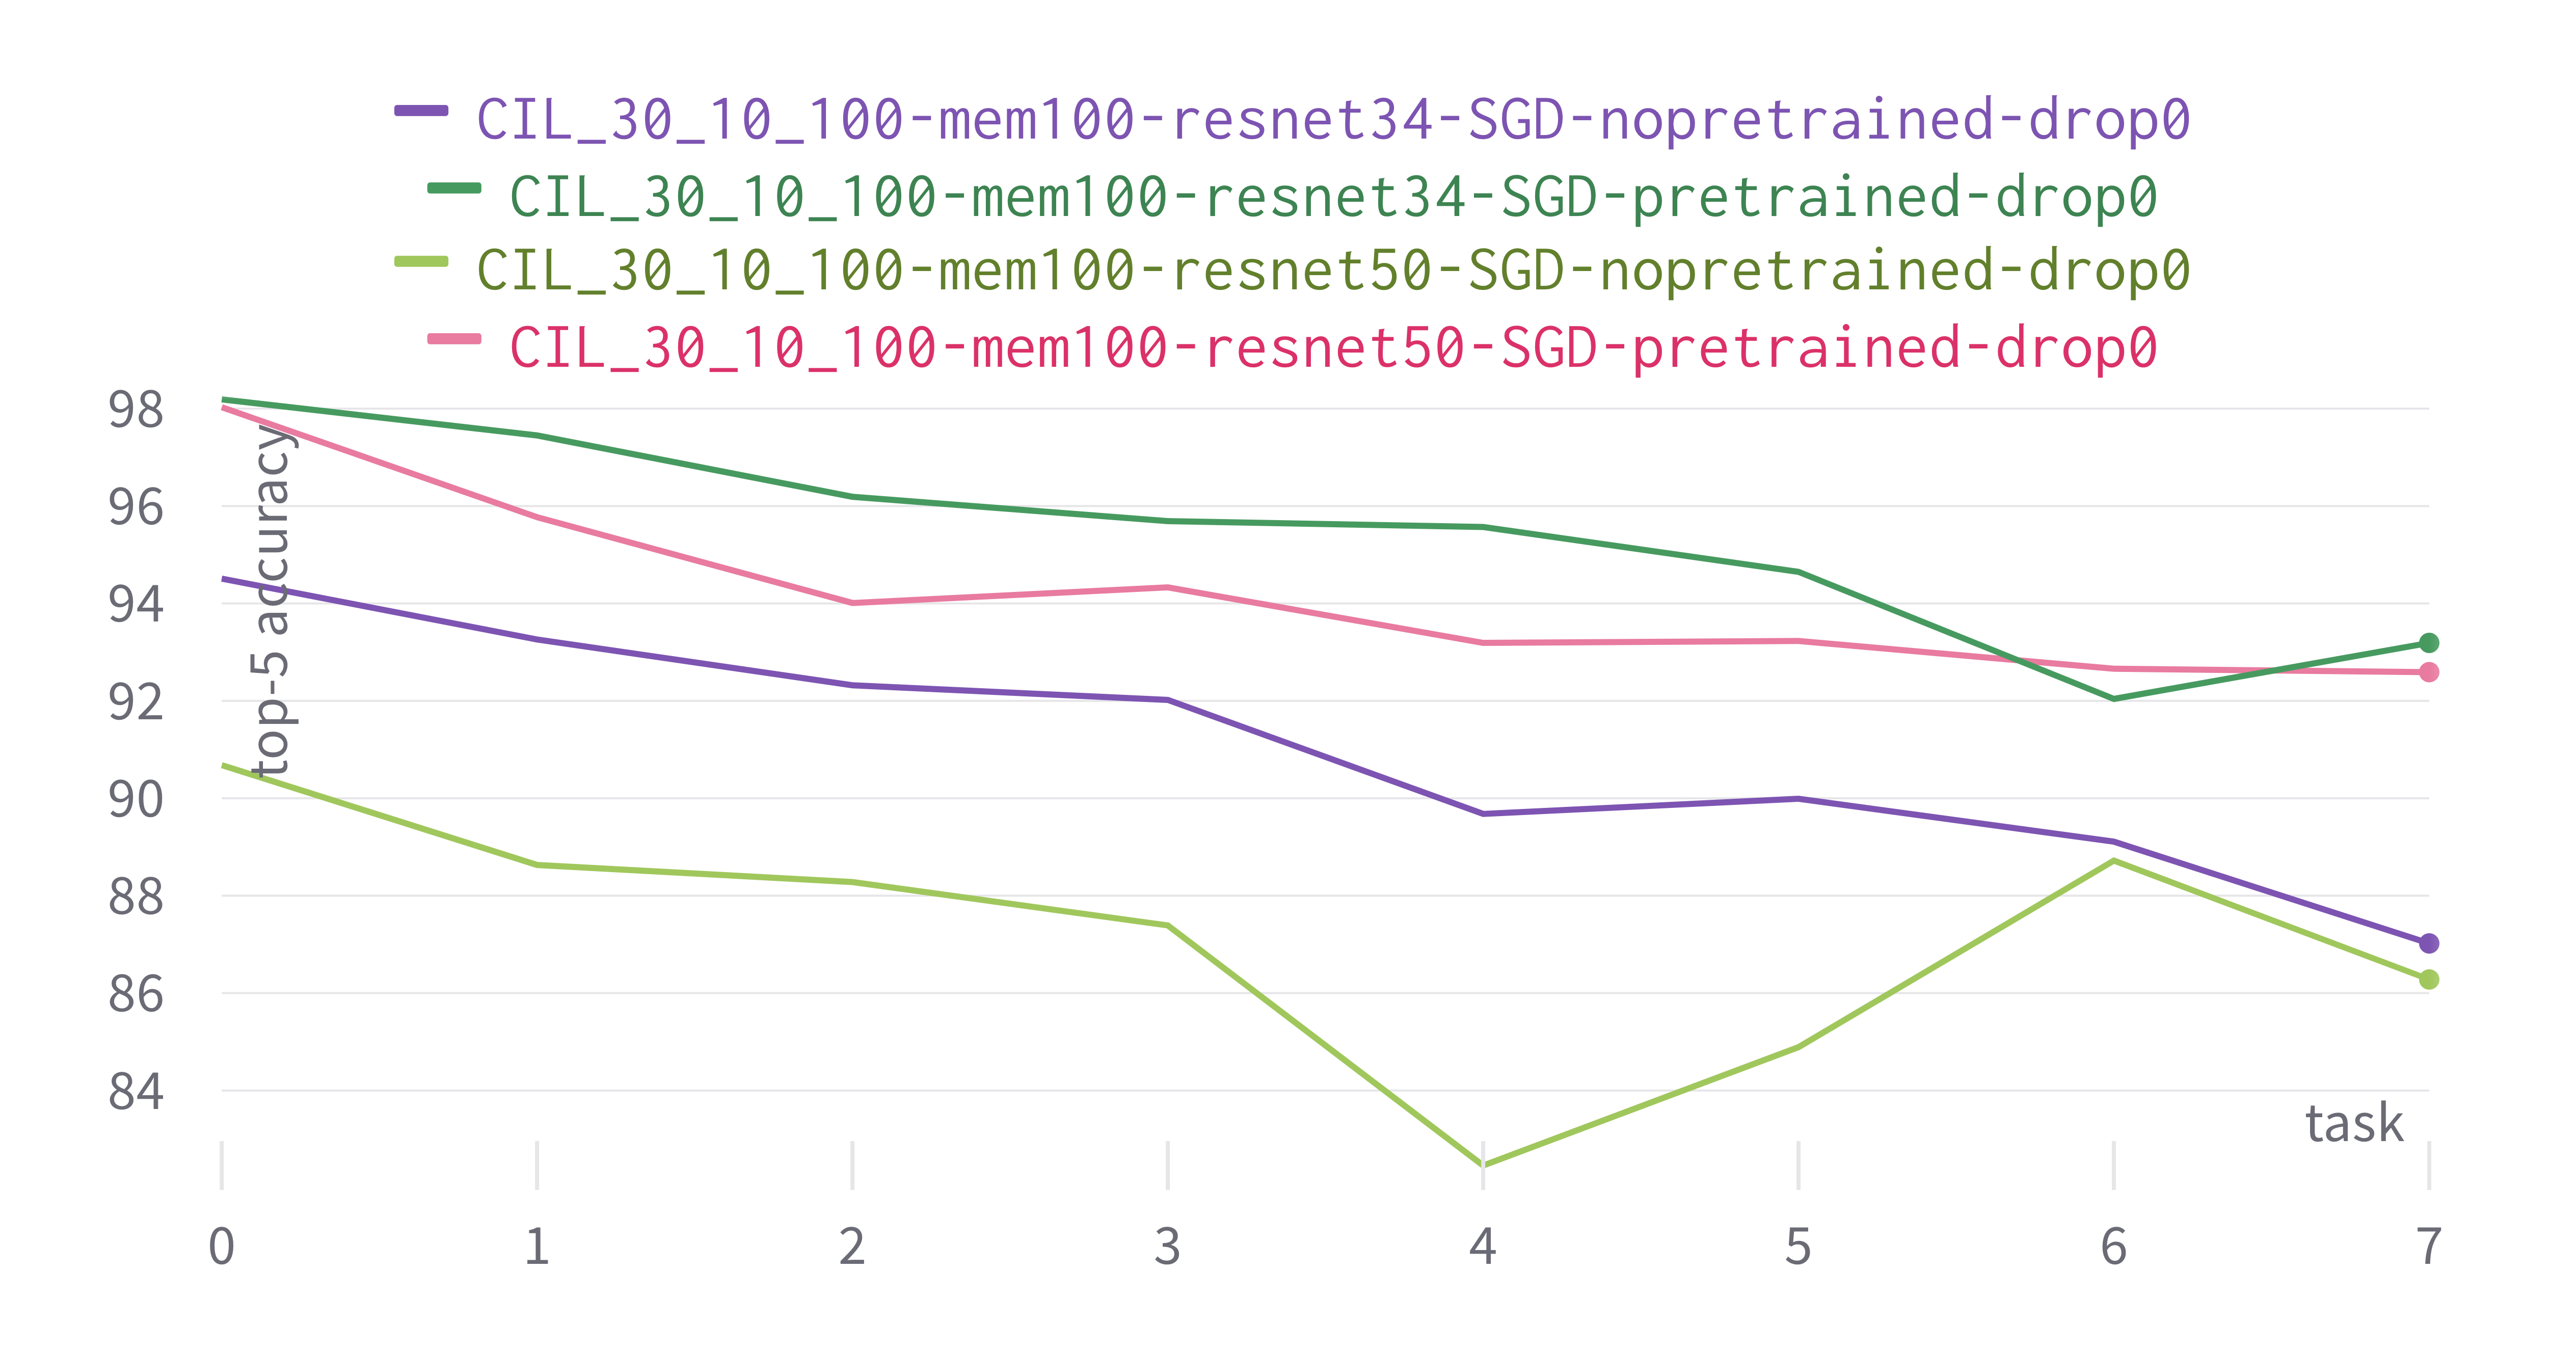
\includegraphics[width=0.50\textwidth]{images/exp/exp1-top5.png} }}%
	\caption{Top-1 and Top-5 accuracy of the models at varying CIL tasks on the test set.}%
	\label{fig:exp1}%
\end{figure}


\begin{table}[H]
    \centering
    \centerline{
    \begin{tabular}{c|c|c|c|c}
        \hline
        \textbf{Name} &
        \textbf{Backbone} &
        \textbf{Pre-trained} &
        \textbf{Top-1} & 
        \textbf{Top-5} \\
        &
        &
        &
        \textbf{acc. (\%)} & 
        \textbf{acc. (\%)} \\
        \hline
        \hline
CIL\_30\_10\_100-mem100-resnet34-SGD-nopretrained-drop0 &ResNet-34&no& 52.97 & 87.02\\
CIL\_30\_10\_100-mem100-resnet34-SGD-pretrained-drop0 &ResNet-34&yes& \textbf{60.37} & \textbf{93.19}\\
CIL\_30\_10\_100-mem100-resnet50-SGD-nopretrained-drop0 &ResNet-50&no& 50.43 & 86.28\\
CIL\_30\_10\_100-mem100-resnet50-SGD-pretrained-drop0 &ResNet-50&yes& 58.54 & 92.59\\
        \hline        
    \end{tabular}}
    \caption{Top-1 and Top-5 accuracy of the models at the task 7.}
    \label{table:exp1}
\end{table}


\begin{figure}[H]
	\centering
	\subfloat[\centering Accuracy on the training set]{{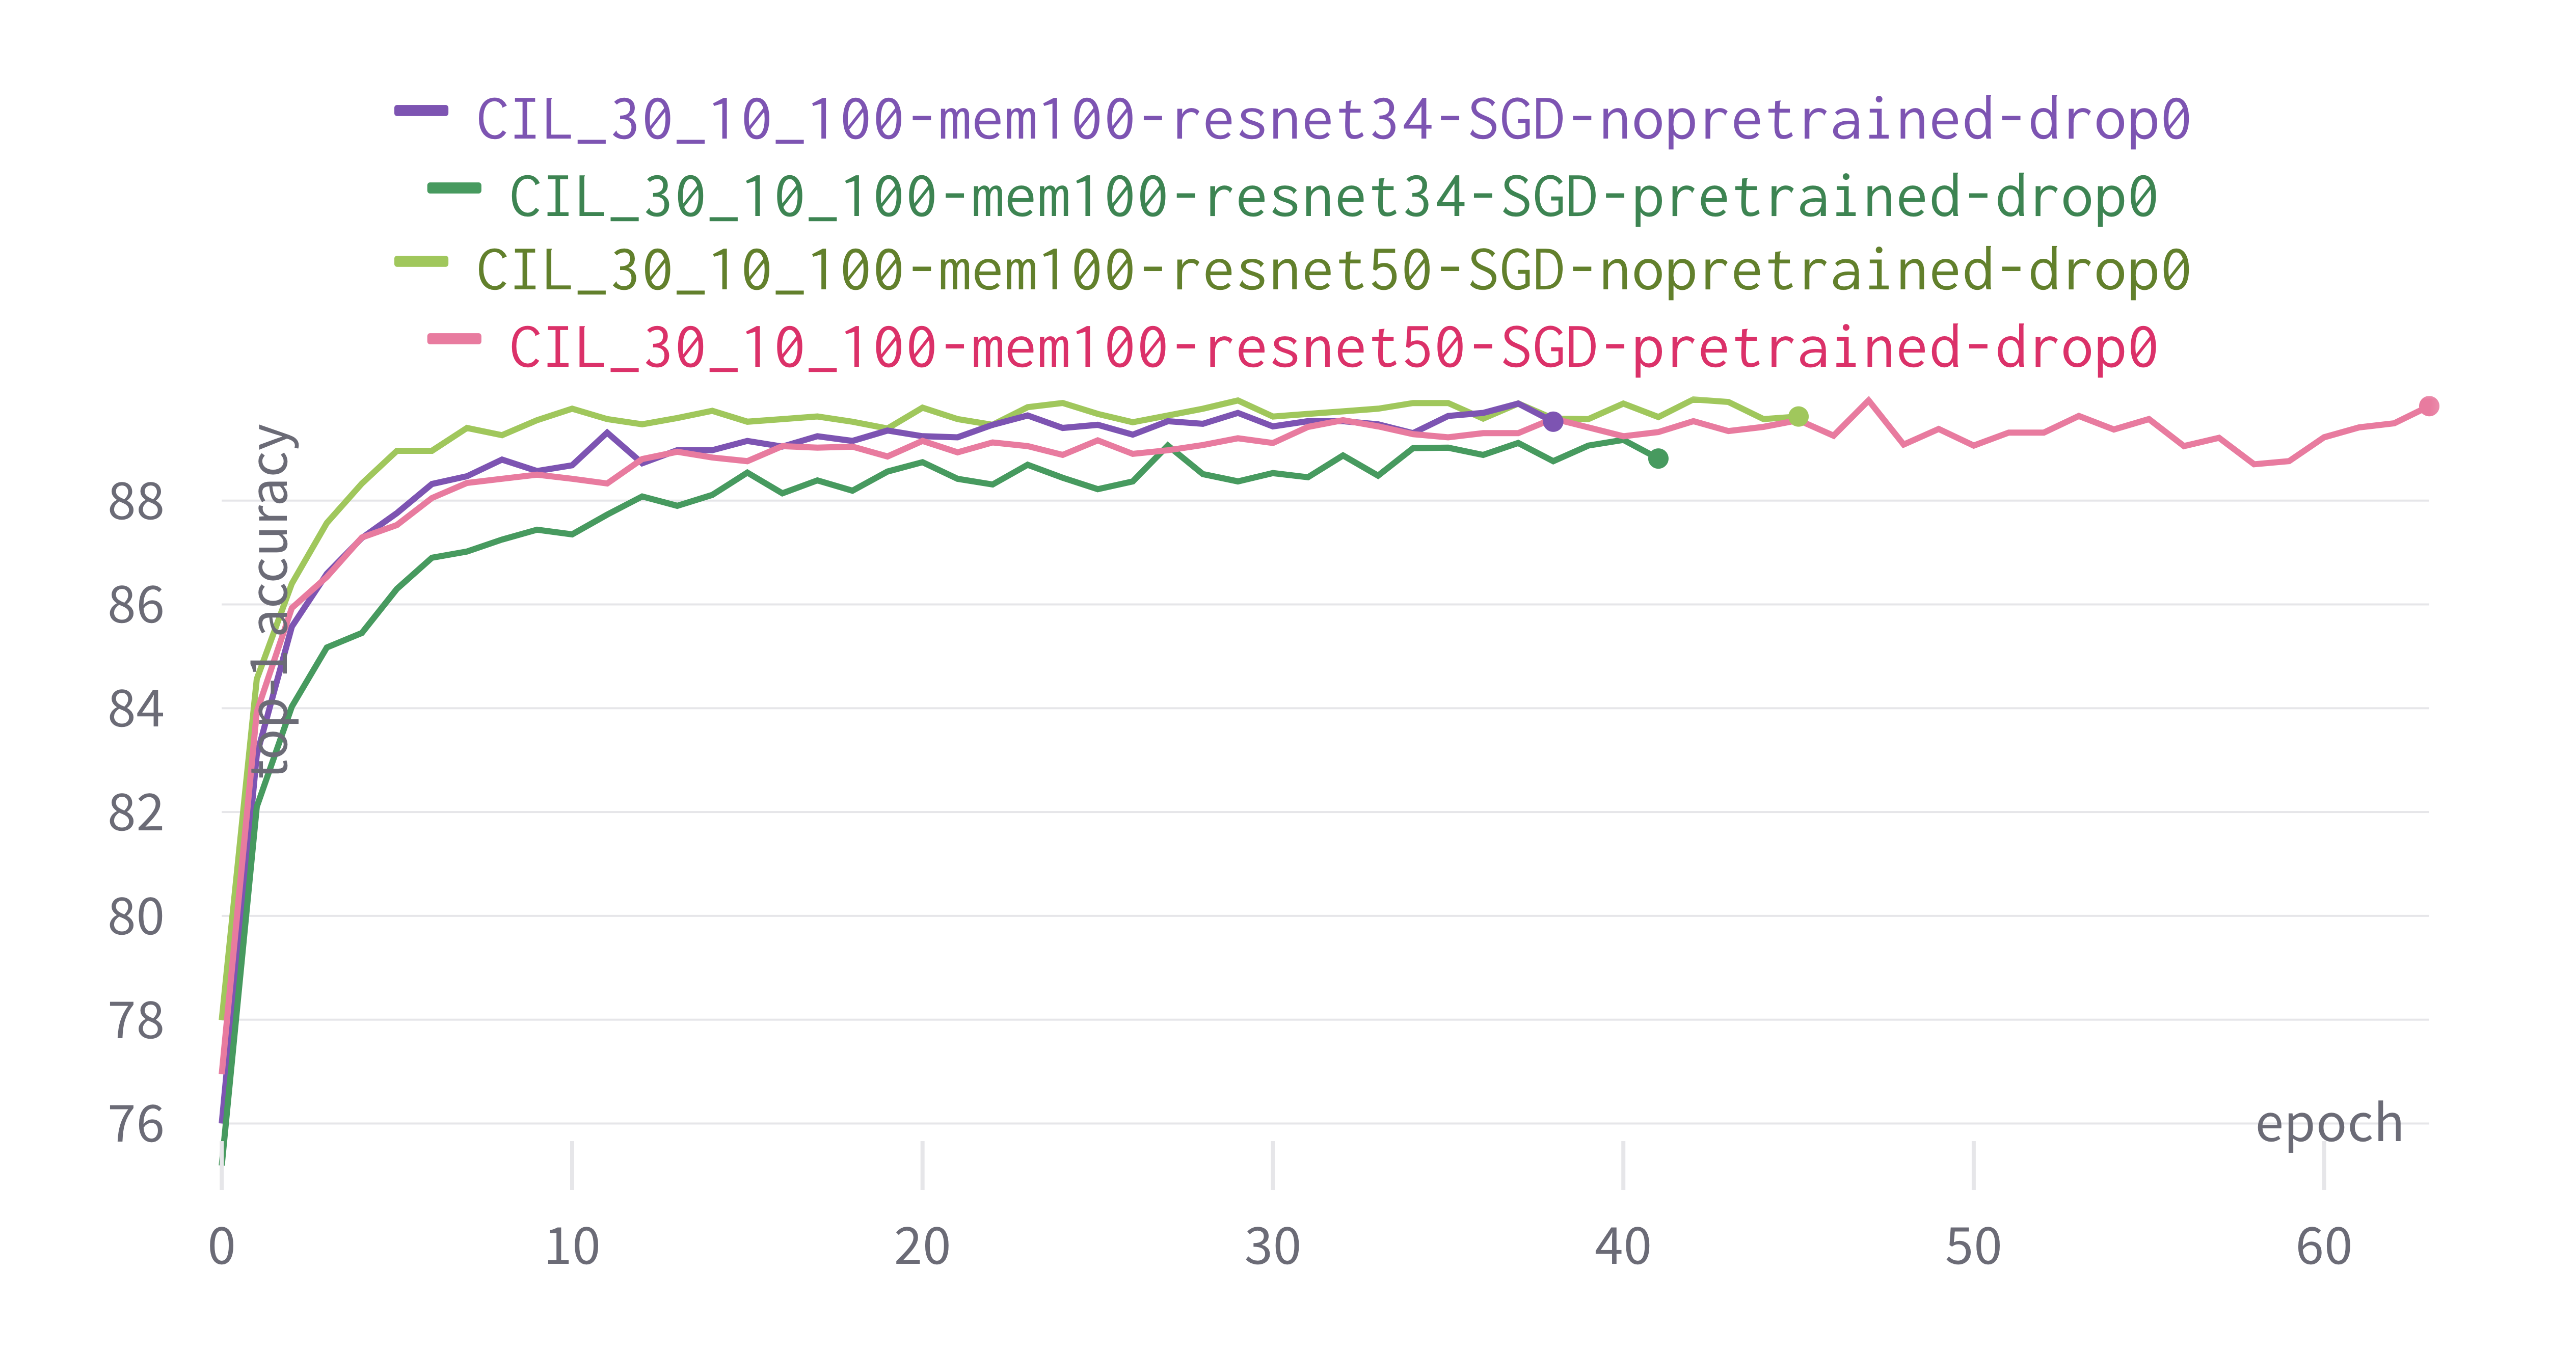
\includegraphics[width=0.49\textwidth]{images/exp/exp1-train.png} }}%
	\subfloat[\centering Accuracy on the validation set]{{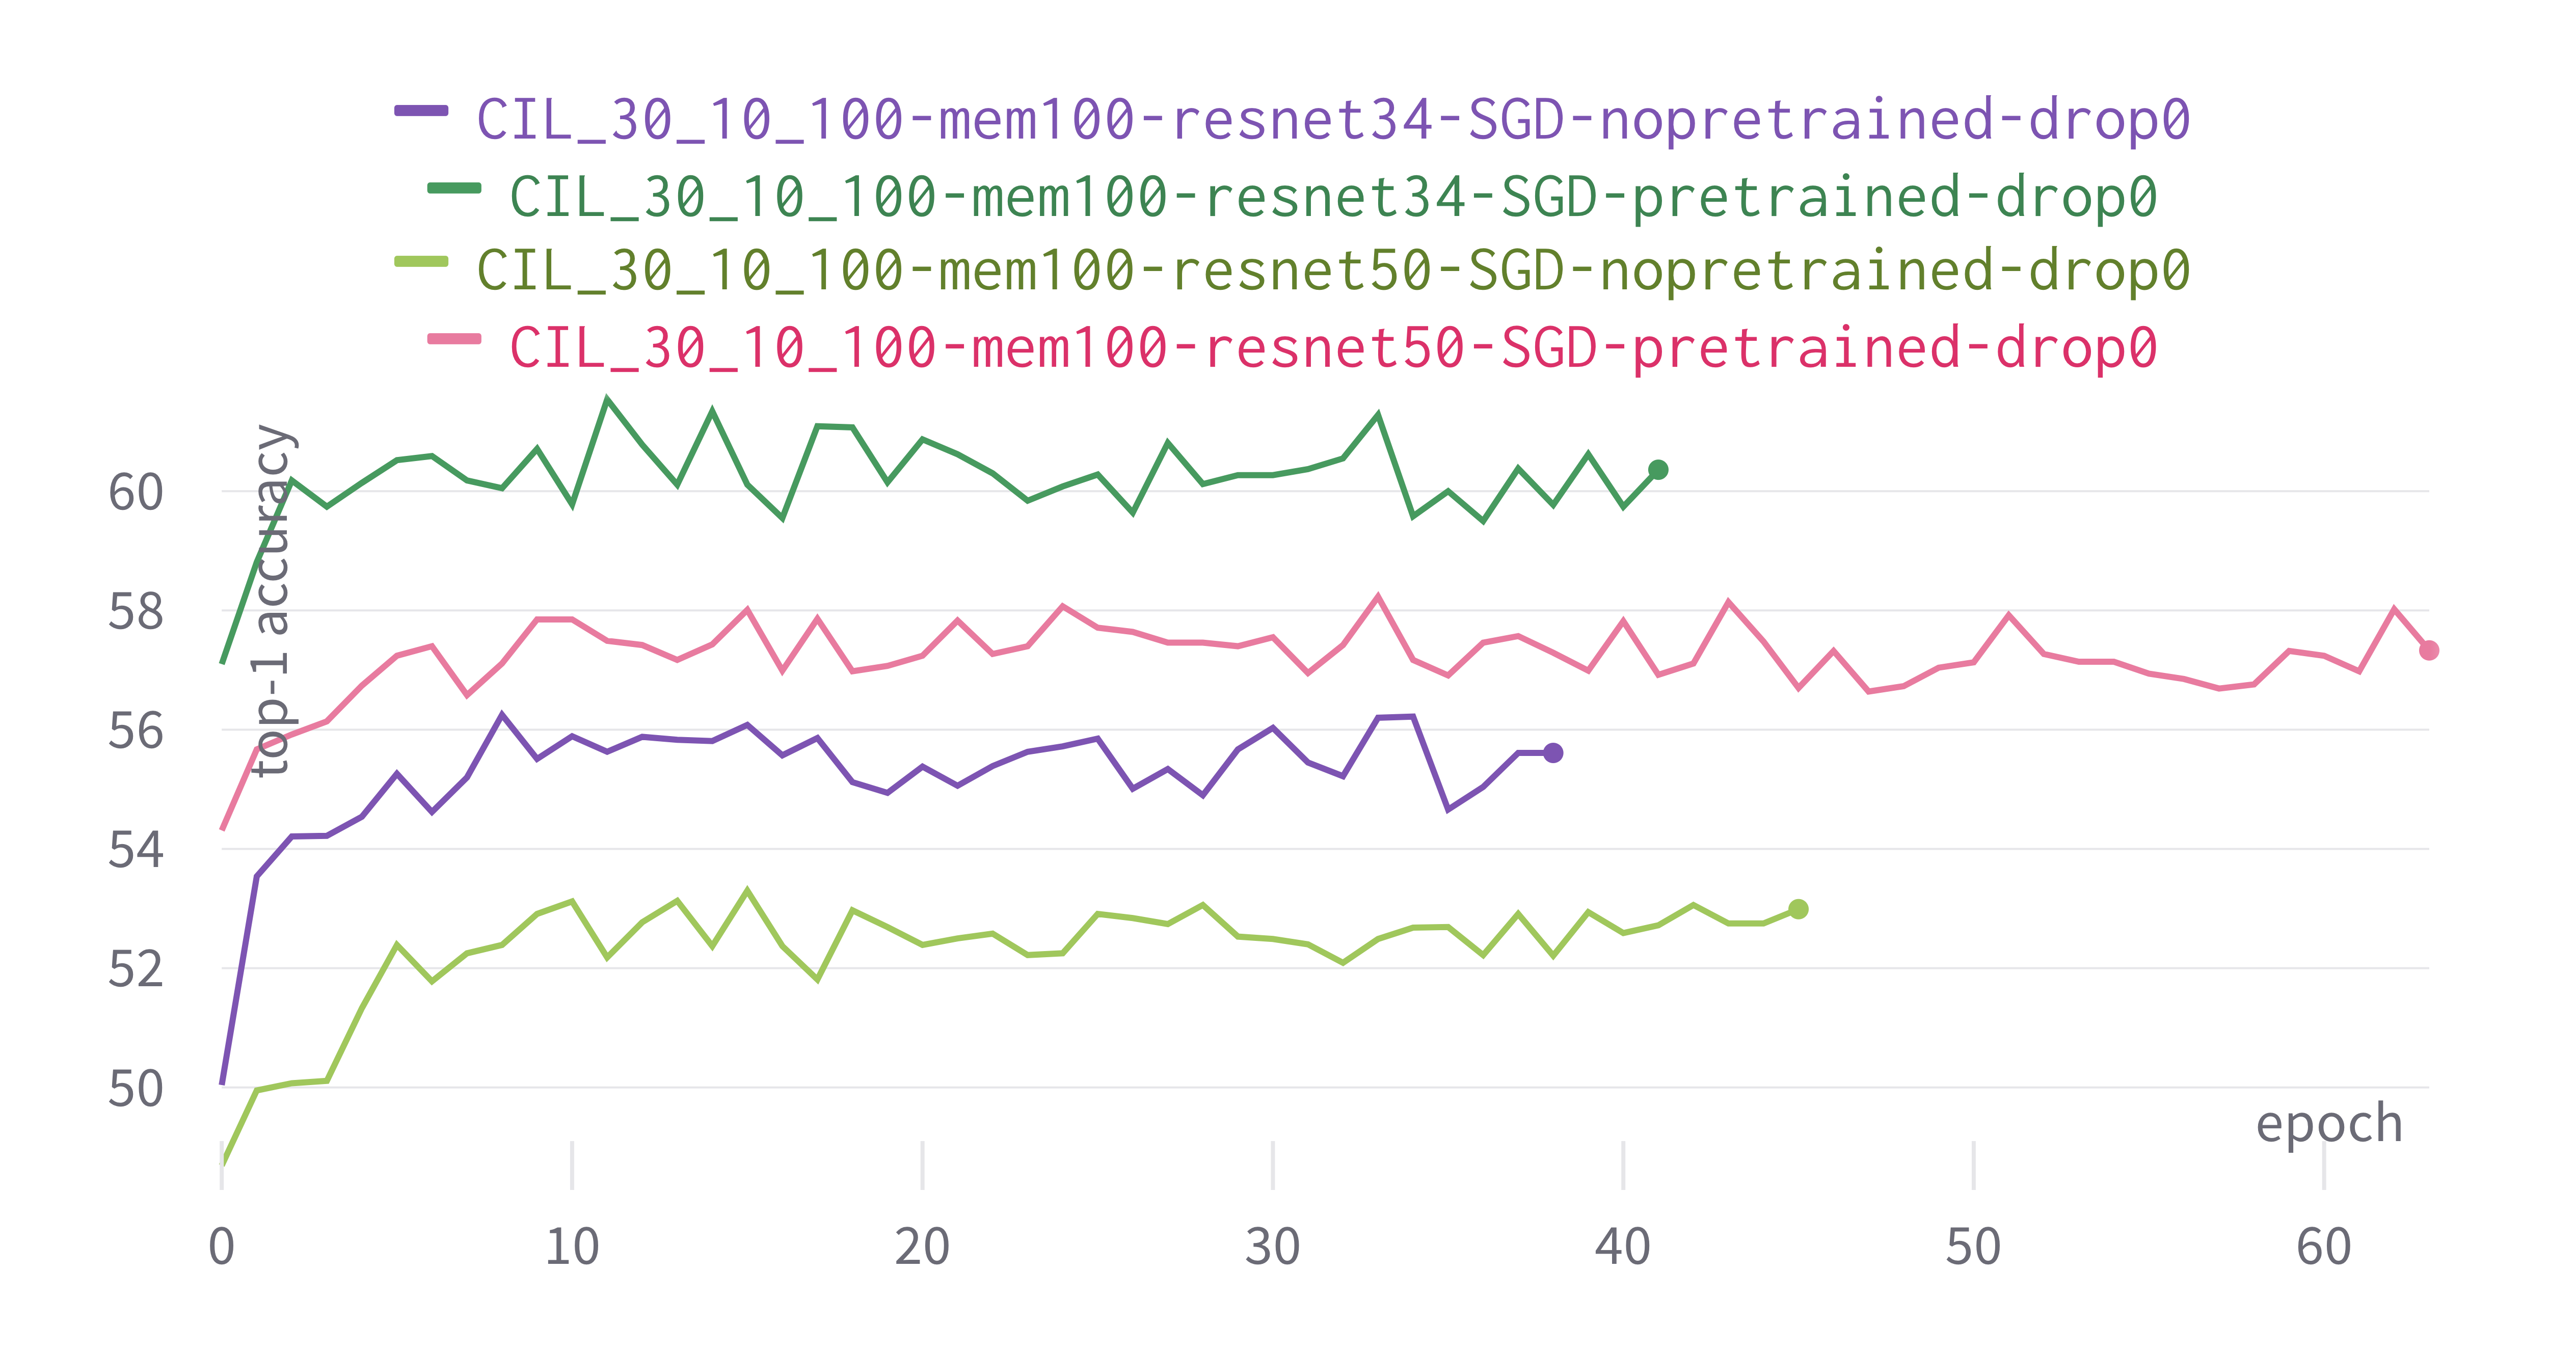
\includegraphics[width=0.49\textwidth]{images/exp/exp1-val.png} }}%
	\caption{Comparison of the accuracy at each training epoch on task 7 between the validation and test set.}%
	\label{fig:exp1-train_val}%
\end{figure}

\subsubsection{Regularization and data augmentation}
Following the analysis discussed above, it is necessary to regularize the model.
To do so, the next experiments are performed using the dropout layer (see \autoref{sec:methods-dropout}) and data augmentation (see \autoref{sec:methods-augment}). As said before, the backbone of each model is ResNet-34 and each one is pre-trained on ImageNet.

As expected, the performance at each task is higher than before, as shown in \autoref{fig:exp2} and in \autoref{table:exp2}. Analyzing \autoref{fig:exp2-train_val}, the accuracy on the train and validation set at task 7 (the same as before), the training accuracy is lower than models without regularization, but the validation accuracy is higher. This is a sign that the regularization works as intended.


\begin{figure}[H]
	\centering
	\subfloat[\centering Top-1 accuracy]{{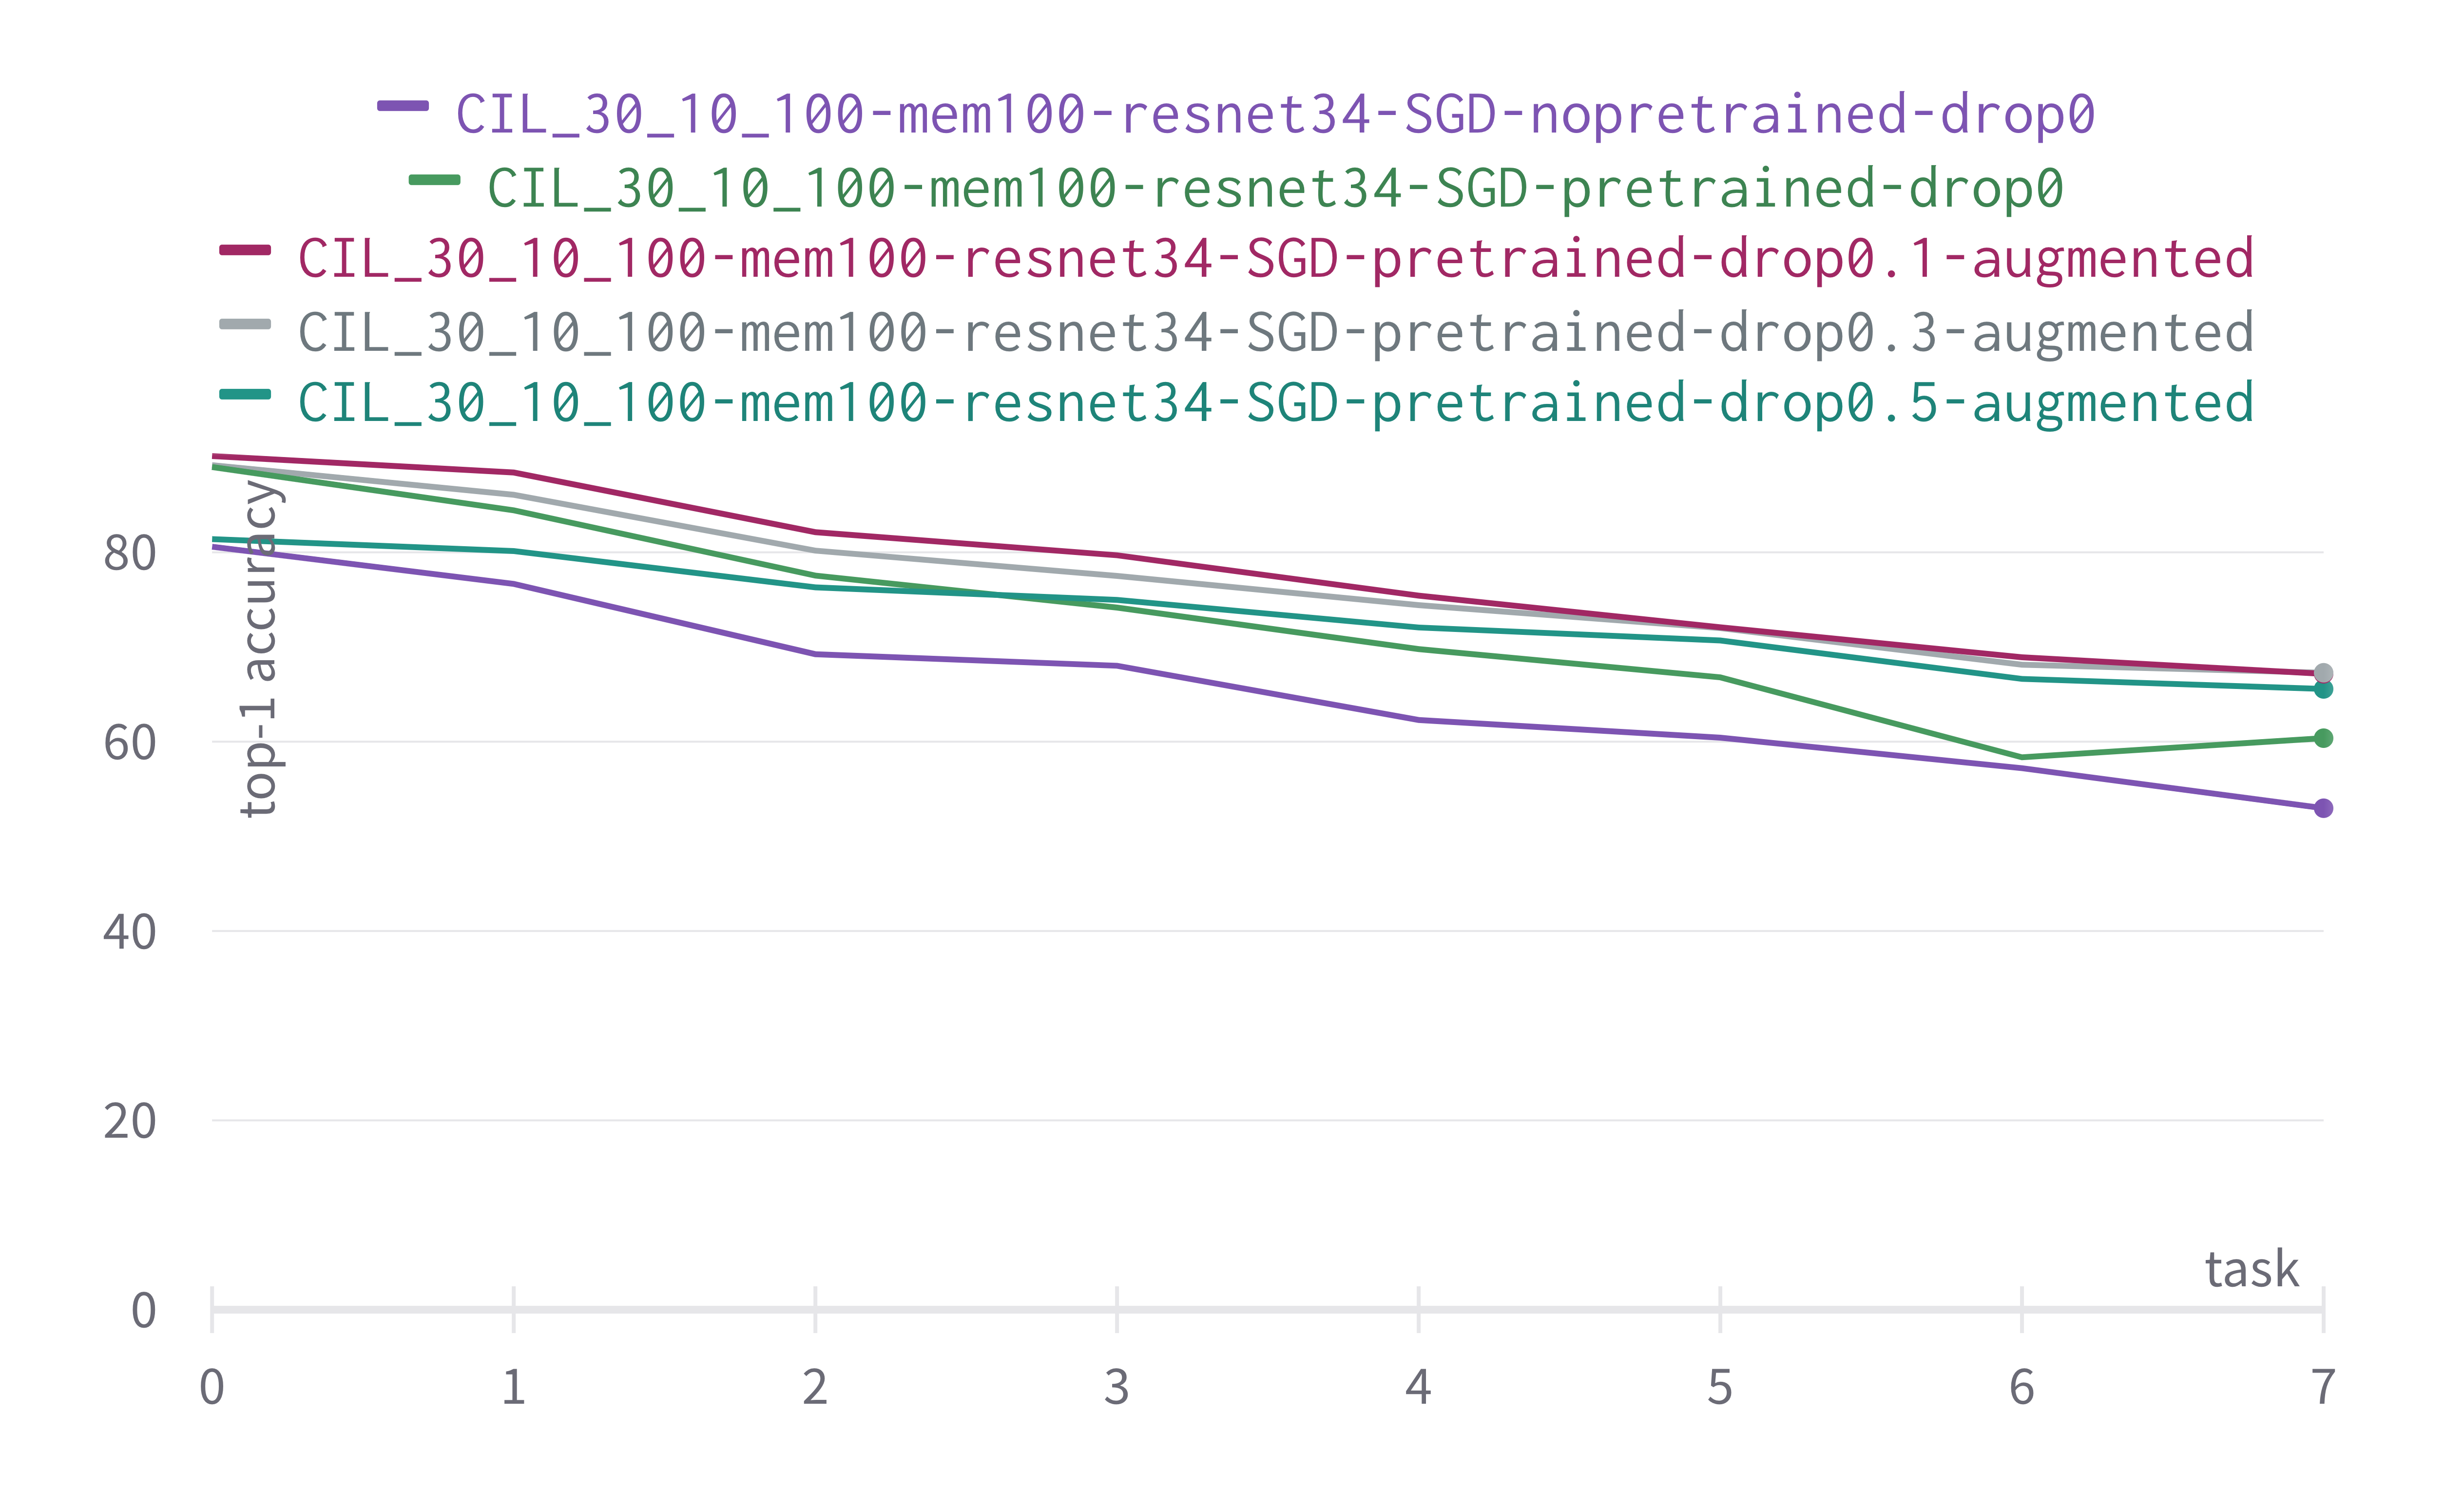
\includegraphics[width=0.50\textwidth]{images/exp/exp2-top1.png} }}%
	\subfloat[\centering Top-5 accuracy]{{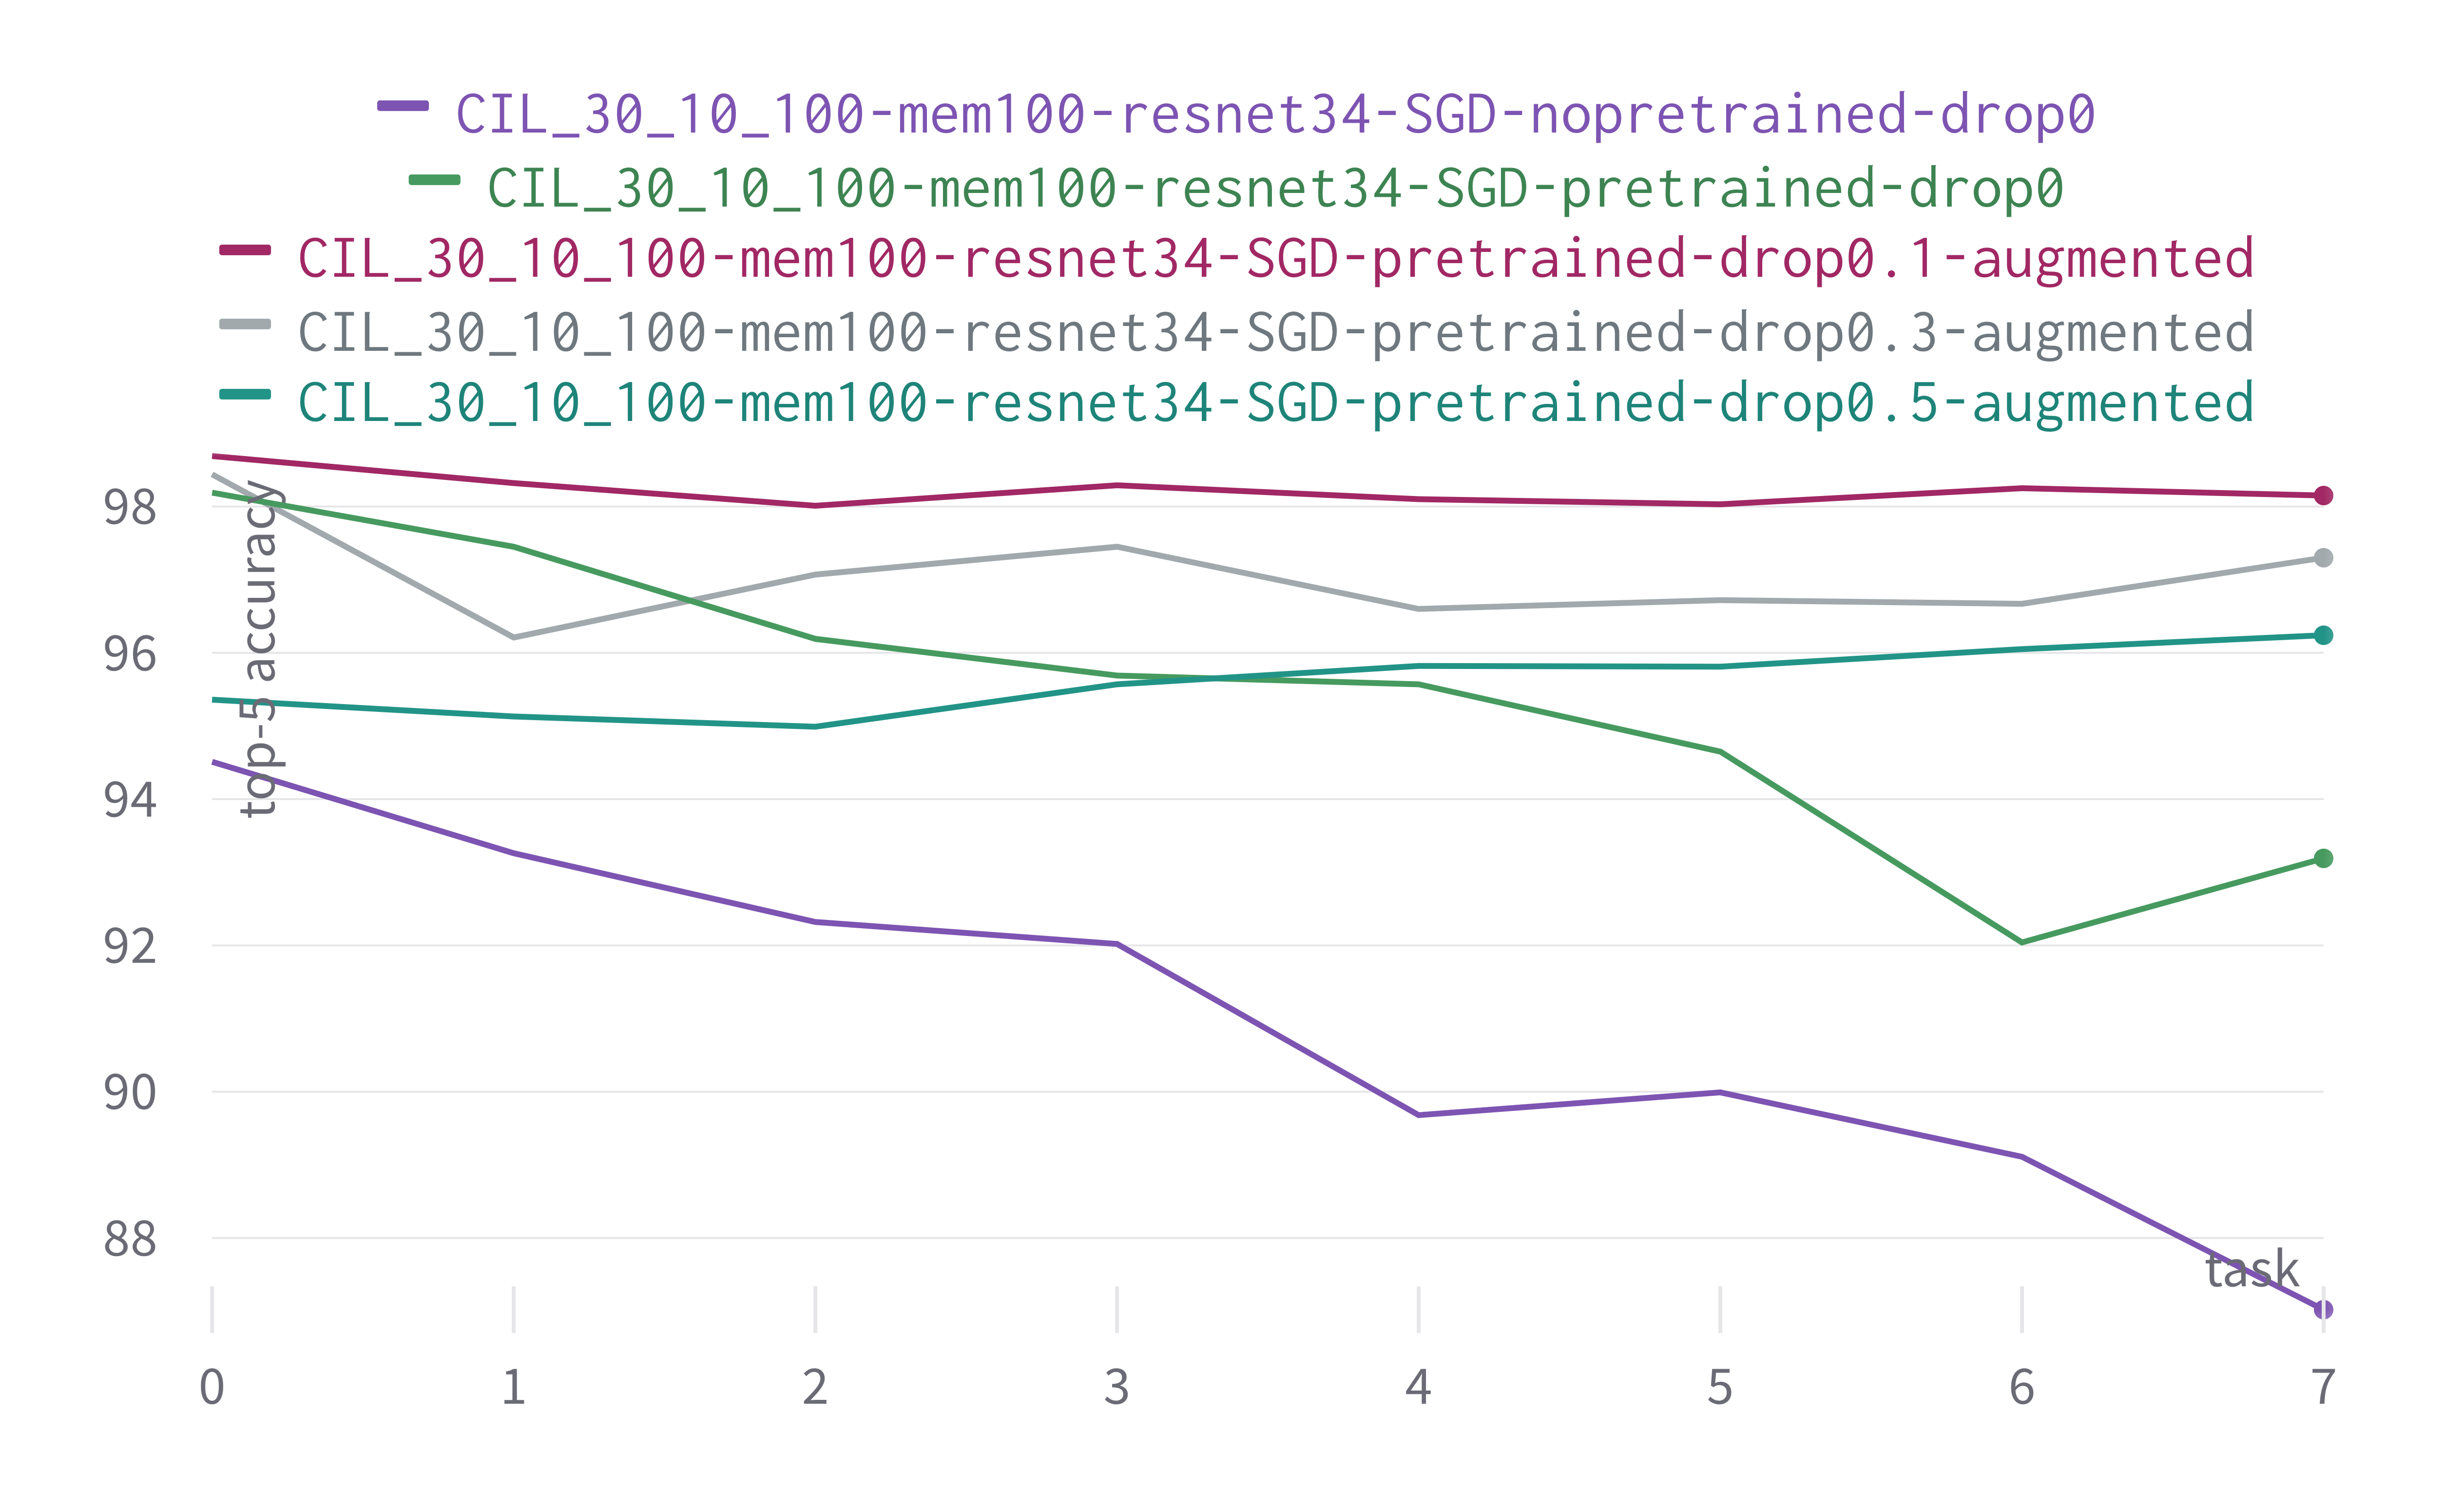
\includegraphics[width=0.50\textwidth]{images/exp/exp2-top5.png} }}%
	\caption{Top-1 and Top-5 accuracy of the regularized models using data augmentation.}%
	\label{fig:exp2}%
\end{figure}



\begin{table}[H]
    \centering
    \centerline{
    \begin{tabular}{c|c|c|c|c}
        \hline
        \textbf{Name} &
        \textbf{Data} &
        \textbf{Dropout} &
        \textbf{Top-1} & 
        \textbf{Top-5} \\
        &
        \textbf{augm.} &
        \textbf{rate} &
        \textbf{acc. (\%)} & 
        \textbf{acc. (\%)} \\
        \hline
        \hline
CIL\_30\_10\_100-mem100-resnet34-SGD-nopretrained-drop0 &no&0.0& 52.97 & 87.02\\
CIL\_30\_10\_100-mem100-resnet34-SGD-pretrained-drop0 &no&0.0& 60.37 & 93.19\\
\hline
CIL\_30\_10\_100-mem100-resnet34-SGD-pretrained-drop0.1-augmented&yes&0.1&	67.17&\textbf{98.15}\\
CIL\_30\_10\_100-mem100-resnet34-SGD-pretrained-drop0.3-augmented&yes&0.3&\textbf{67.28}&	97.3\\
CIL\_30\_10\_100-mem100-resnet34-SGD-pretrained-drop0.5-augmented&yes&0.5&65.57&	96.24\\
        \hline        
    \end{tabular}}
    \caption{Regularized models with data augmentation. Top-1 and Top-5 accuracy at the task 7.}
    \label{table:exp2}
\end{table}

\begin{figure}[H]
	\centering
	\subfloat[\centering Accuracy on the training set]{{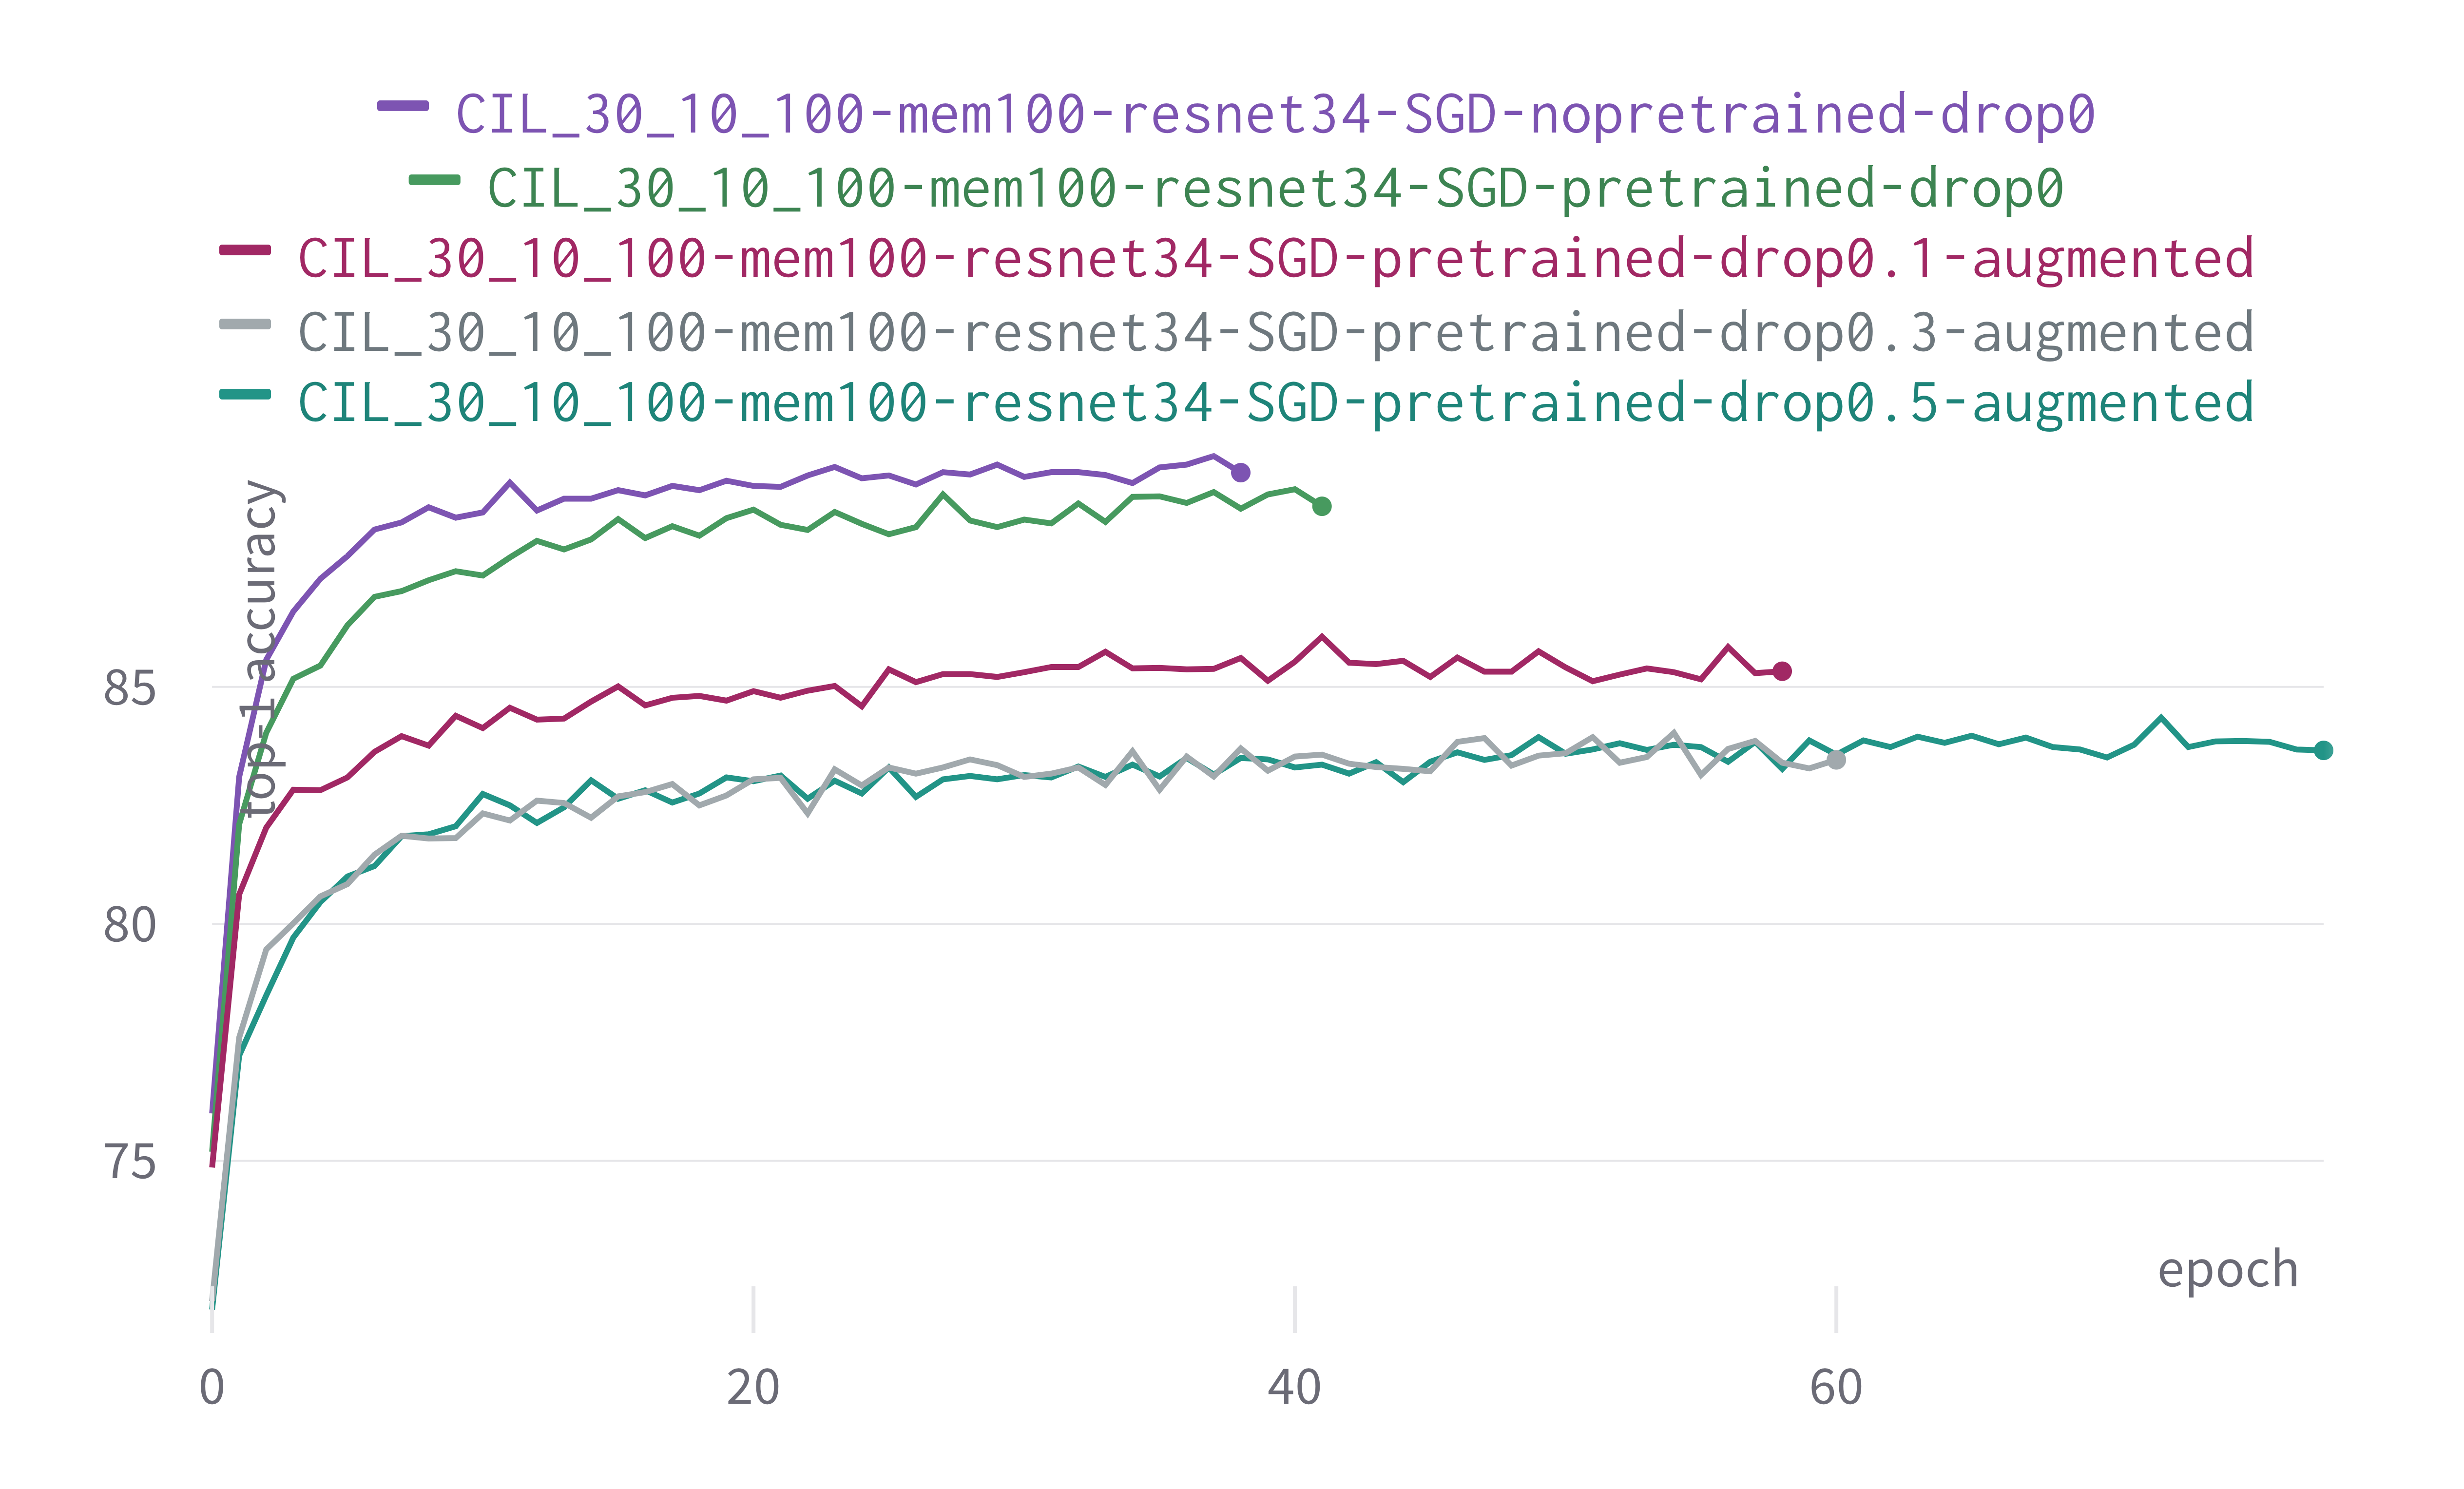
\includegraphics[width=0.49\textwidth]{images/exp/exp2-train.png} }}%
	\subfloat[\centering Accuracy on the validation set]{{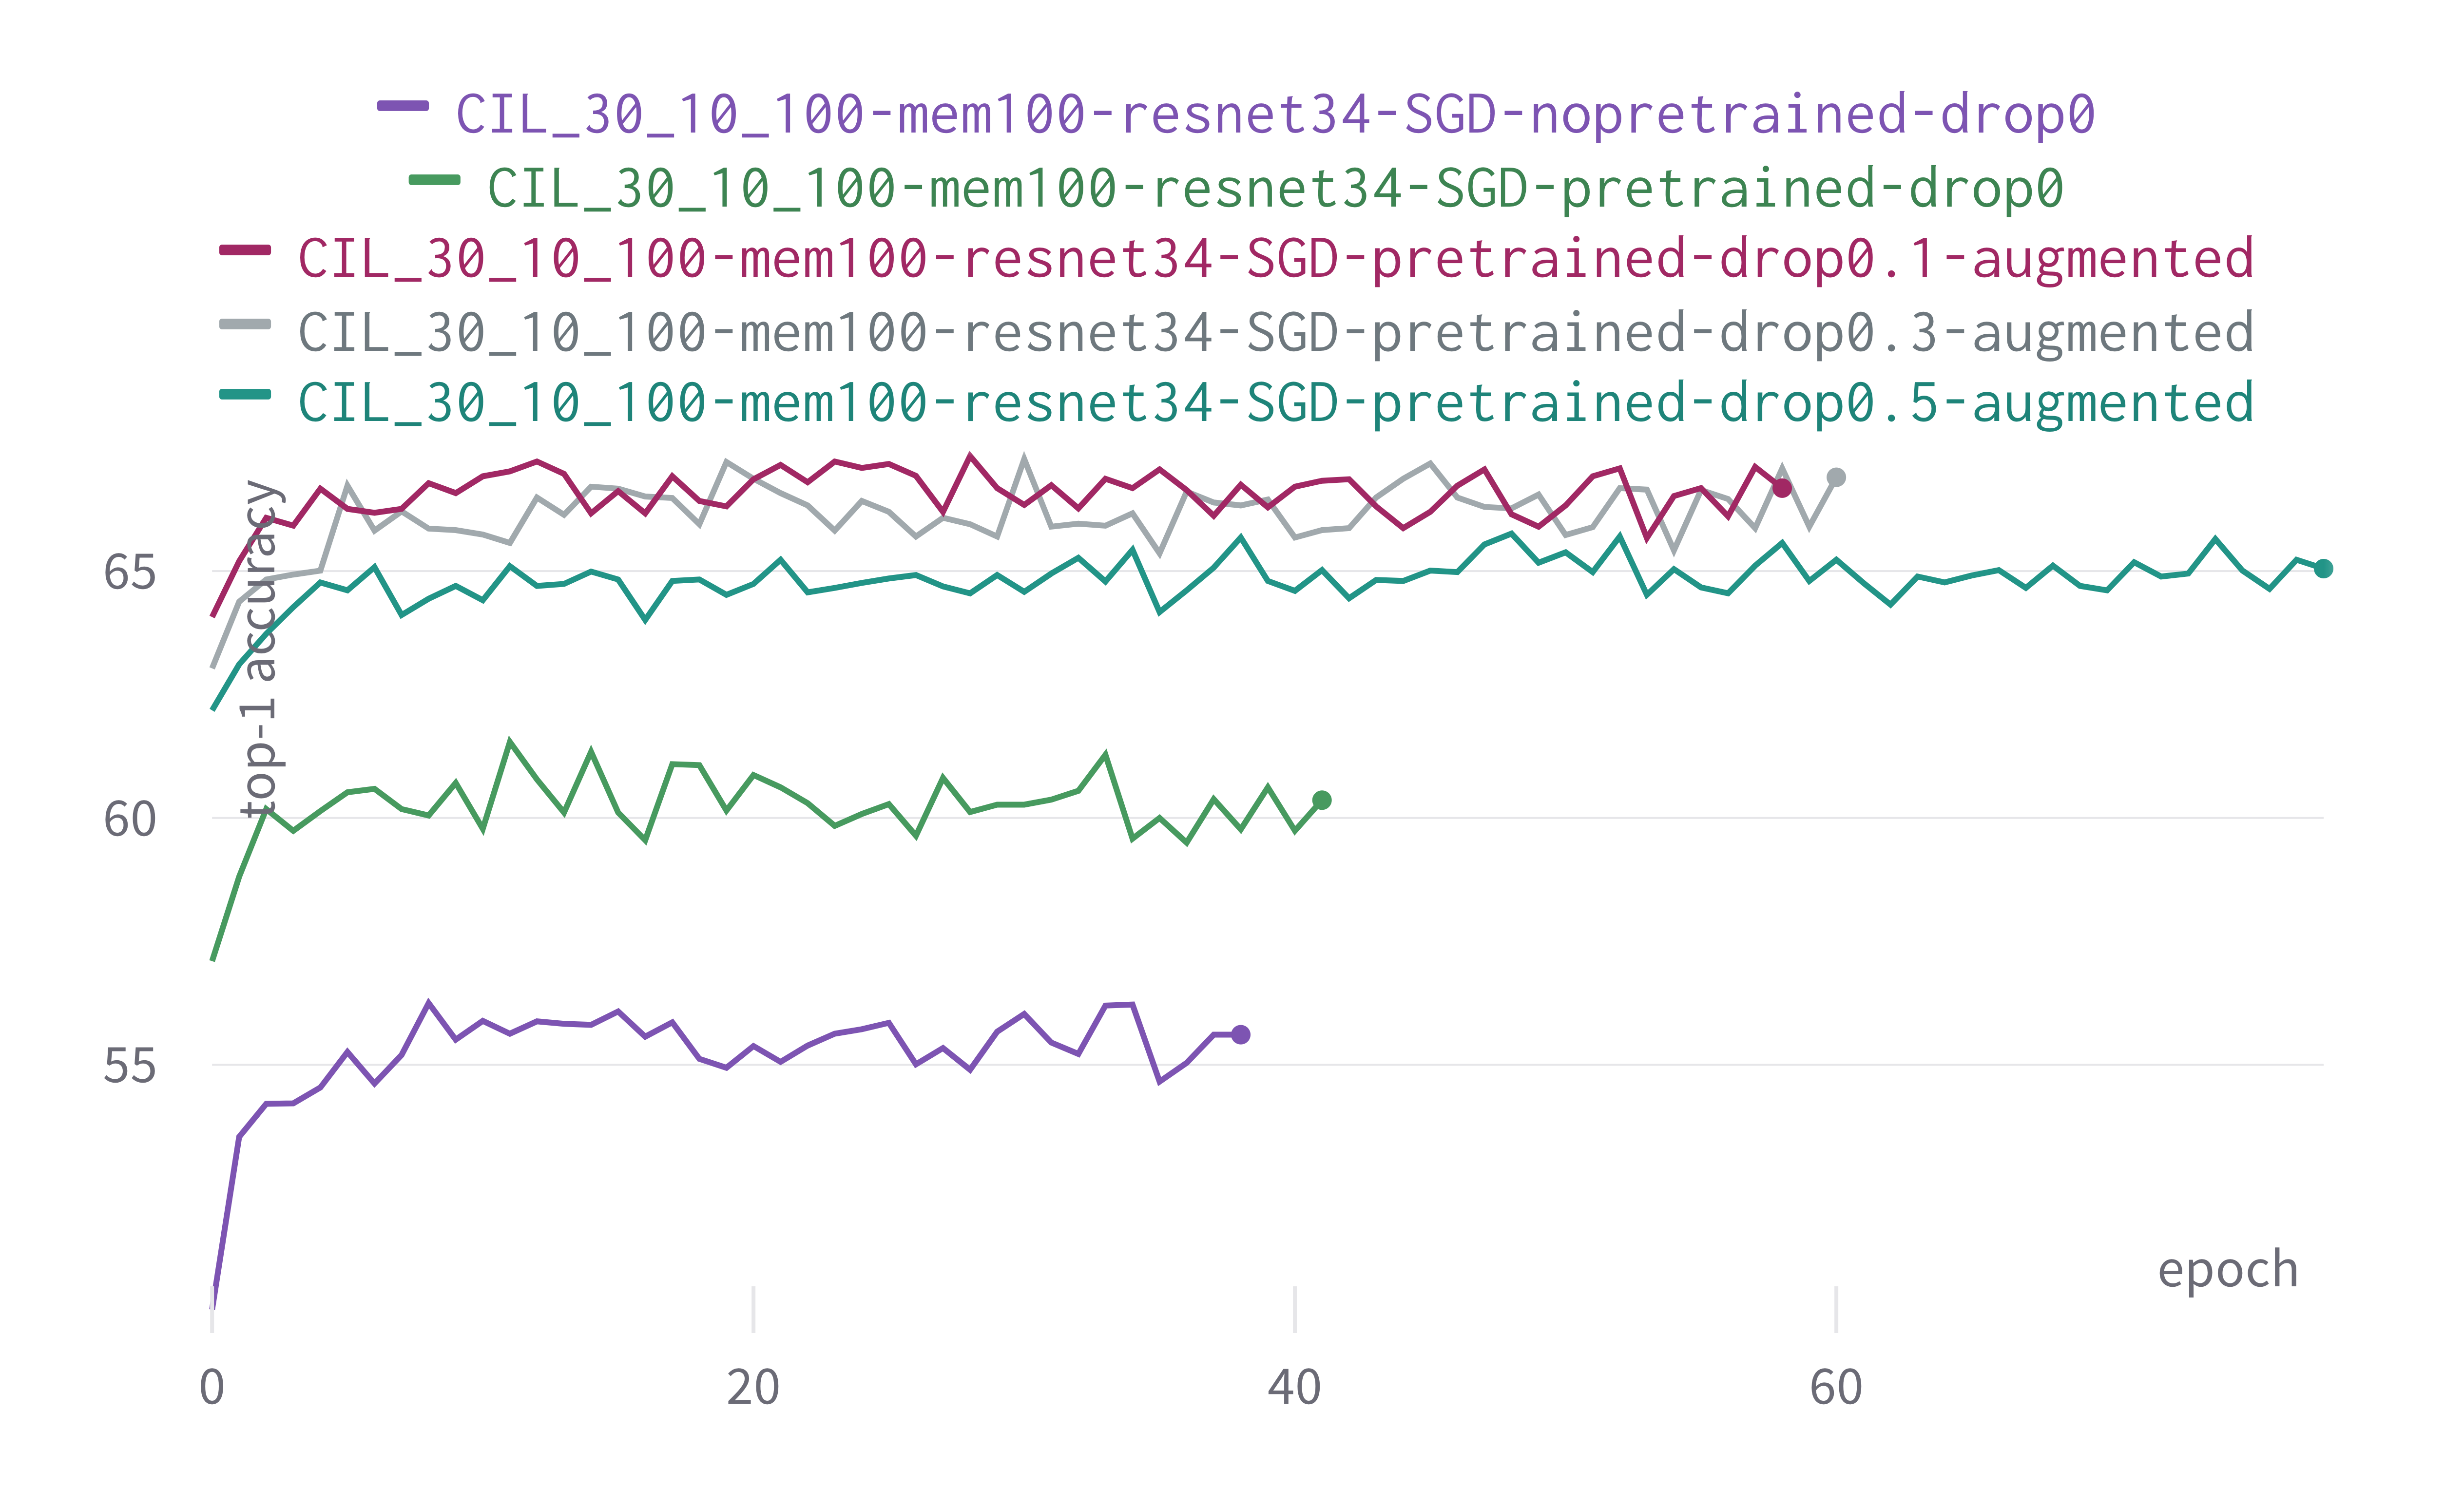
\includegraphics[width=0.49\textwidth]{images/exp/exp2-val.png} }}%
	\caption{Regularized models with data augmentation: comparison of the accuracy at each training epoch on task 7 between the validation and test set.}%
	\label{fig:exp2-train_val}%
\end{figure}


\subsubsection{Introduction of Adam optimizer}

\subsection{2993 Classes}
\label{sec:whole_dataset_clf}
\section{Logo detector}
\label{sec:exp-det}
\subsection{Metrics}
\subsection{100 Classes}
\subsection{2993 Classes}
\subsubsection{Ablation study}
WA non utilizzato ma non peggiora molto le cose, probabilemnte perchè ci sono pochi esempi quindi qeusto non affect molto.

\section{Knowledge Distillation}
\label{sec:exp-kd}
\section{End to end classification}
\label{sec:exp-end2end}

% 700x400 vs 600x300 (small)